\subsubsection{UC 14 - Eliminare una cartella} \label{sec:UC14}
    \begin{itemize}
        \item \textbf{Attore principale}: MUA;
        \item \textbf{Descrizione}: il MUA elimina una cartella dal sistema;
        \item \textbf{Precondizioni}: il MUA sta usando la funzionalità di eliminazione di un oggetto;
        \item \textbf{Postcondizioni}: il sistema elimina la cartella con l'identificativo fornito dal MUA;
        \item \textbf{Scenario principale}:
            \begin{enumerate}
                \item il MUA invia i dettagli della cartella da eliminare al sistema (\hyperref[sec:UC14.1]{UC 14.1});
                \item il sistema elimina la cartella;
            \end{enumerate}
        \item \textbf{Inclusioni}: nessuna;
        \item \textbf{Generalizzazioni}: nessuna;
        \item \textbf{Estensioni}: nessuna.
    \end{itemize}

\begin{figure}[h]
    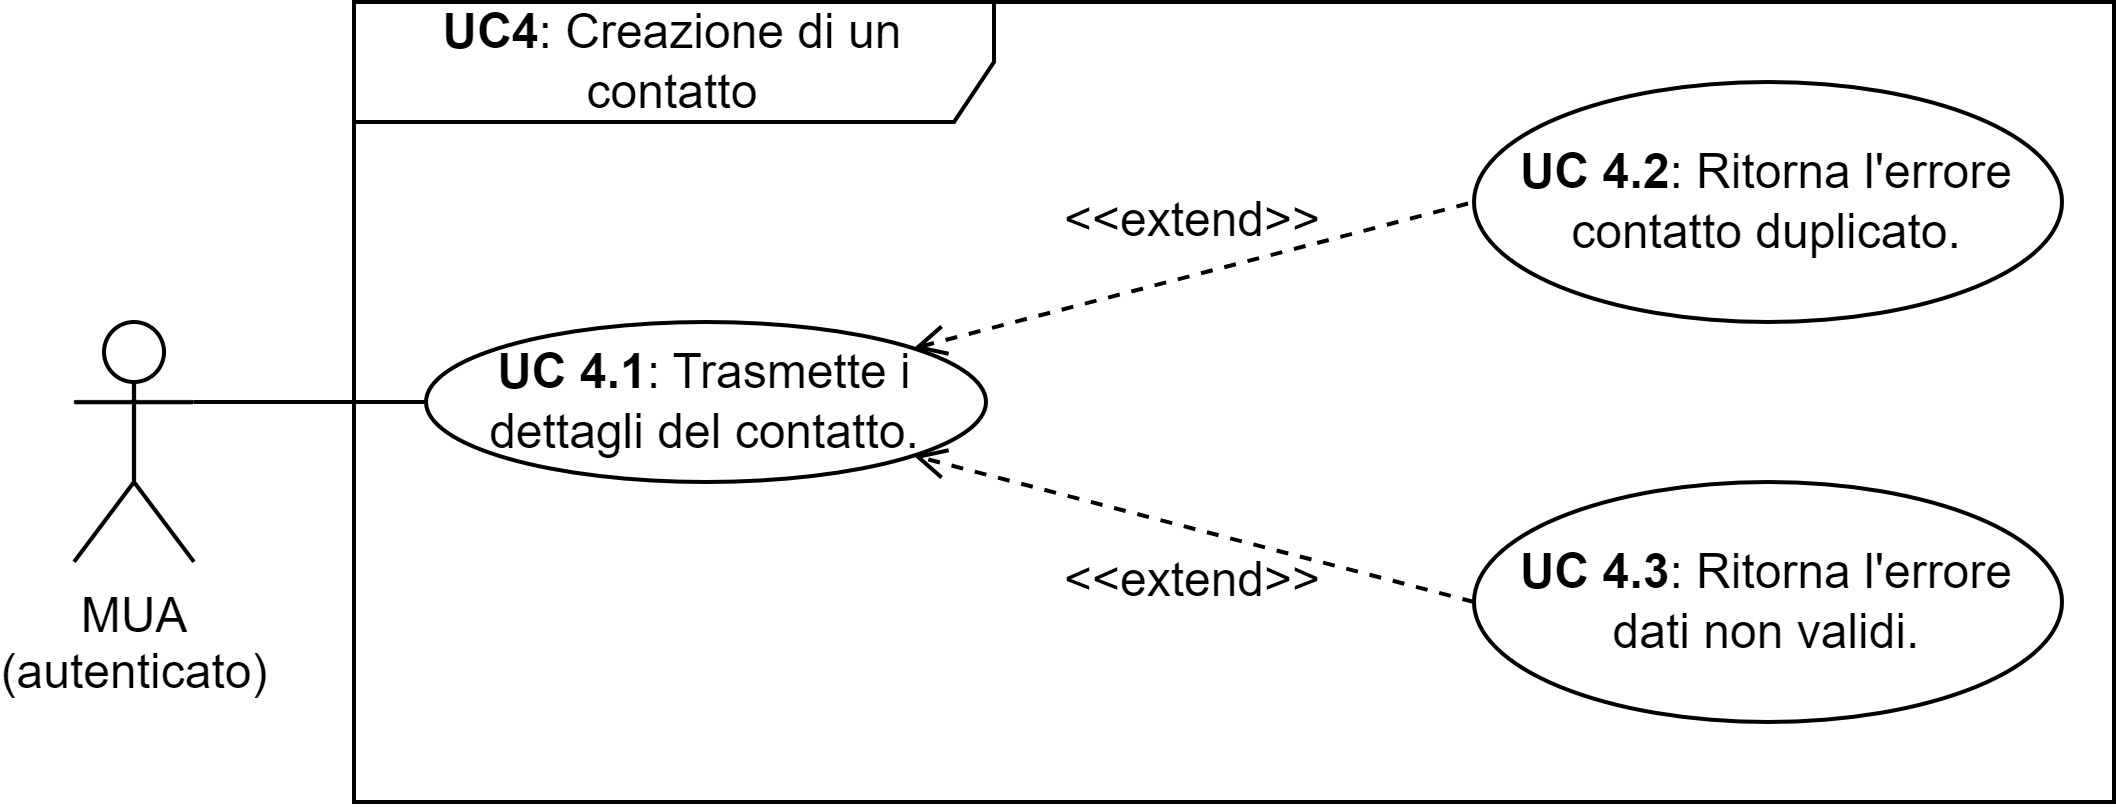
\includegraphics[width=0.85\textwidth]{sections/uc_imgs/UC04.X.png}
    \centering
    \caption{Diagramma sotto-casi UC 14.}
\end{figure}

\subsubsection{UC 14.1 - Trasmette i dettagli della cartella} \label{sec:UC14.1}
    \begin{figure}[h]
        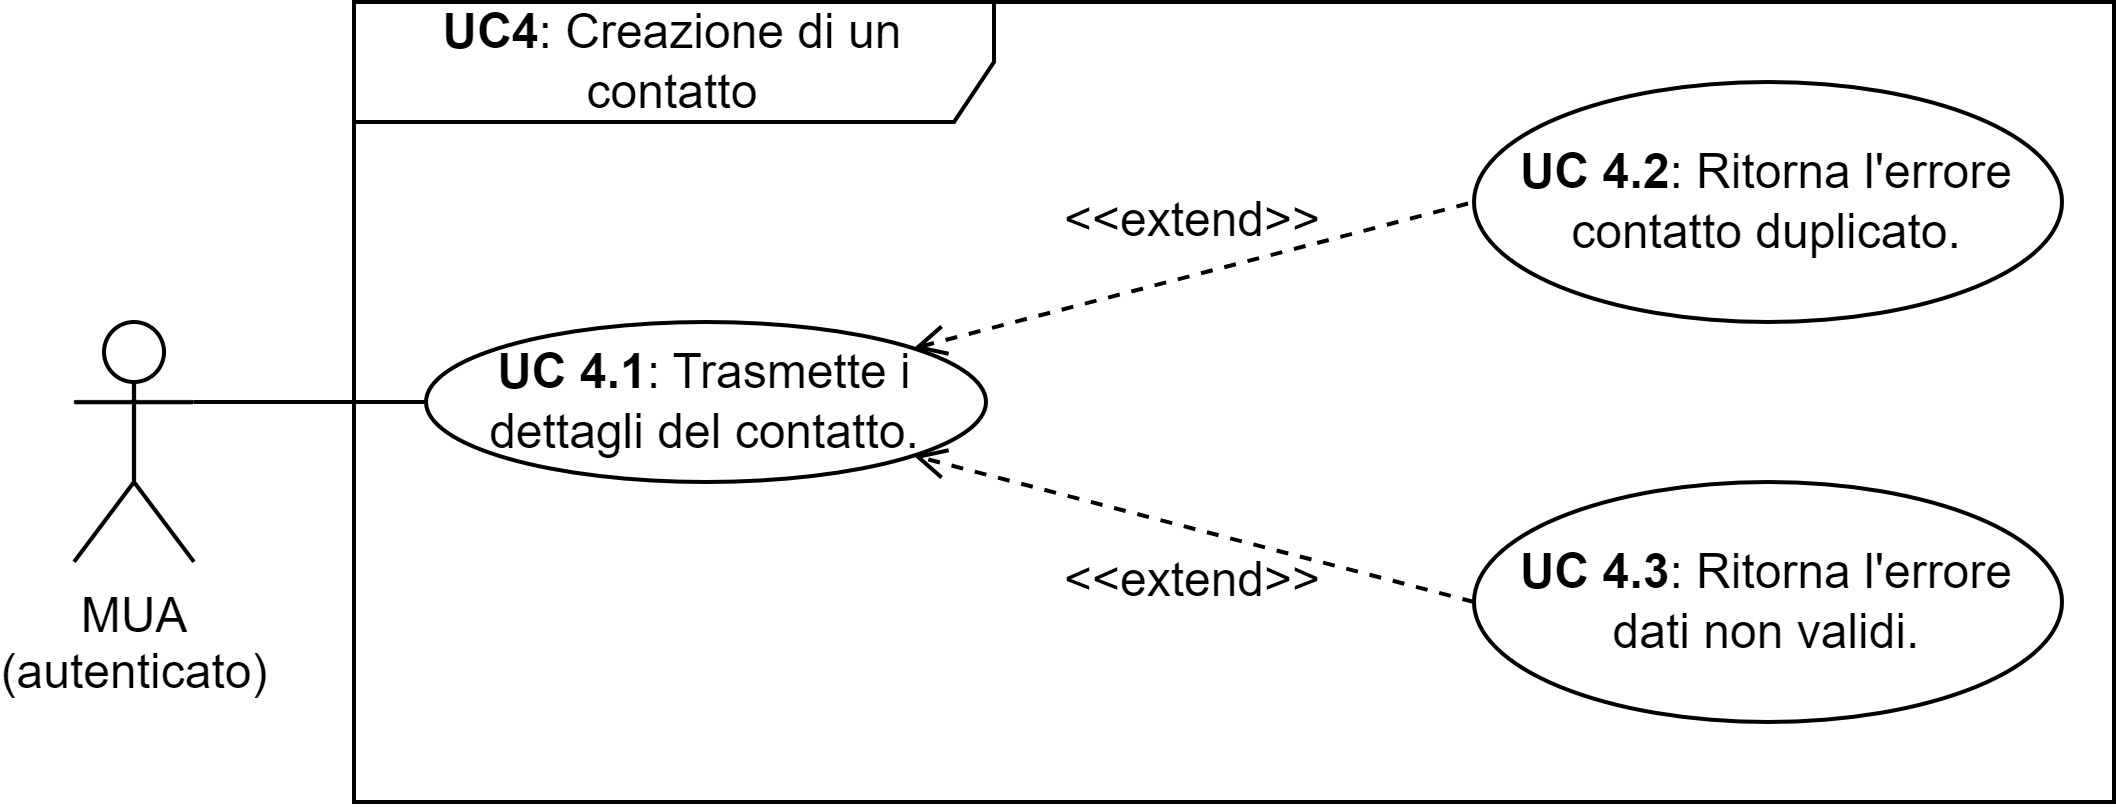
\includegraphics[width=0.85\textwidth]{sections/uc_imgs/UC04.X.png}
        \centering
        \caption{Diagramma UC 14.1.}
    \end{figure}
    \begin{itemize}
        \item \textbf{Attore principale}: MUA;
        \item \textbf{Descrizione}: il MUA invia le informazioni della cartella da eliminare al sistema;
        \item \textbf{Precondizioni}: il MUA sta usando la funzionalità di eliminazione di una cartella;
        \item \textbf{Postcondizioni}: il sistema elimina la cartella identificata dalle informazioni fornite dal MUA;
        \item \textbf{Scenario principale}:
            \begin{enumerate}
                \item il MUA invia l'identificativo della cartella al sistema;
                \item il sistema controlla che la cartella identificata rispetti i seguenti requisiti:
                \begin{itemize}
                    \item la cartella non contiene altre email;
                    \item la cartella non contiene altre cartelle;
                \end{itemize}
            \end{enumerate}
        \item \textbf{Inclusioni}: nessuna;
        \item \textbf{Generalizzazioni}: nessuna;
        \item \textbf{Estensioni}:
            \begin{enumerate}[label=\alph*.]
                \item il sistema non riesce a eliminare la cartella perché non è stata trovata:
                \begin{enumerate}[label=\arabic*.]
                    \item il sistema ritorna un errore al MUA di identificativo non valido (\hyperref[sec:UC14.2]{UC 14.2}).
                \end{enumerate}
                \item il sistema non riesce a eliminare la cartella perché contiene delle email:
                \begin{enumerate}[label=\arabic*.]
                    \item il sistema ritorna un errore al MUA di cartella contenente email (\hyperref[sec:UC14.3]{UC 14.3}).
                \end{enumerate}
                \item il sistema non riesce a eliminare la cartella perché contiene altre cartelle:
                \begin{enumerate}[label=\arabic*.]
                    \item il sistema ritorna un errore al MUA di cartella contenente cartelle (\hyperref[sec:UC14.4]{UC 14.4}).
                \end{enumerate}
            \end{enumerate}
    \end{itemize}


\subsubsection{UC 14.2 - Ricezione errore identificativo cartella non valida} \label{sec:UC14.2}
    \begin{itemize}
        \item \textbf{Attore principale}: MUA;
        \item \textbf{Descrizione}: il sistema non riesce a eliminare la cartella perché l'identificativo cartella non è stato trovato;
        \item \textbf{Precondizioni}: il MUA sta usando la funzionalità d'invio dei dettagli al sistema di una cartella;
        \item \textbf{Postcondizioni}: il sistema non elimina la cartella, il MUA è stato notificato dell'errore;
        \item \textbf{Scenario principale}:
            \begin{enumerate}
                \item il sistema non trova la cartella con l'identificativo fornito dal MUA;
                \item il sistema non elimina la cartella e notifica il MUA dell'errore;
            \end{enumerate}
        \item \textbf{Inclusioni}: nessuna;
        \item \textbf{Generalizzazioni}: nessuna;
        \item \textbf{Estensioni}: nessuna.
    \end{itemize}
   
    \subsubsection{UC 14.3 - Ricezione errore cartella contenente email} \label{sec:UC14.3}

    \begin{itemize}
        \item \textbf{Attore principale}: MUA;
        \item \textbf{Descrizione}: il sistema non riesce a eliminare la cartella perché una o più email sono presenti all'interno di quella cartella;
        \item \textbf{Precondizioni}: il MUA sta usando la funzionalità d'invio dei dettagli al sistema di una cartella;
        \item \textbf{Postcondizioni}: il sistema non elimina la cartella, il MUA è stato notificato dell'errore;
        \item \textbf{Scenario principale}:
            \begin{enumerate}
                \item la cartella non soddisfa il requisito di non conetenere email;
                \item il sistema non elimina la cartella e notifica il MUA dell'errore;
            \end{enumerate}
        \item \textbf{Inclusioni}: nessuna;
        \item \textbf{Generalizzazioni}: nessuna;
        \item \textbf{Estensioni}: nessuna.
    \end{itemize}


    \subsubsection{UC 14.4 - Ricezione errore cartella contenente cartelle} \label{sec:UC14.4}

    \begin{itemize}
        \item \textbf{Attore principale}: MUA;
        \item \textbf{Descrizione}: il sistema non riesce a eliminare la cartella perché una o più cartelle sono presenti all'interno di quella cartella;
        \item \textbf{Precondizioni}: il MUA sta usando la funzionalità d'invio dei dettagli al sistema di una cartella;
        \item \textbf{Postcondizioni}: il sistema non elimina la cartella, il MUA è stato notificato dell'errore;
        \item \textbf{Scenario principale}:
            \begin{enumerate}
                \item la cartella non soddisfa il requisito di non conetenere altre cartelle;
                \item il sistema non elimina la cartella e notifica il MUA dell'errore;
            \end{enumerate}
        \item \textbf{Inclusioni}: nessuna;
        \item \textbf{Generalizzazioni}: nessuna;
        \item \textbf{Estensioni}: nessuna.
    \end{itemize}

